

\tikzset{every picture/.style={line width=0.75pt}} %set default line width to 0.75pt        

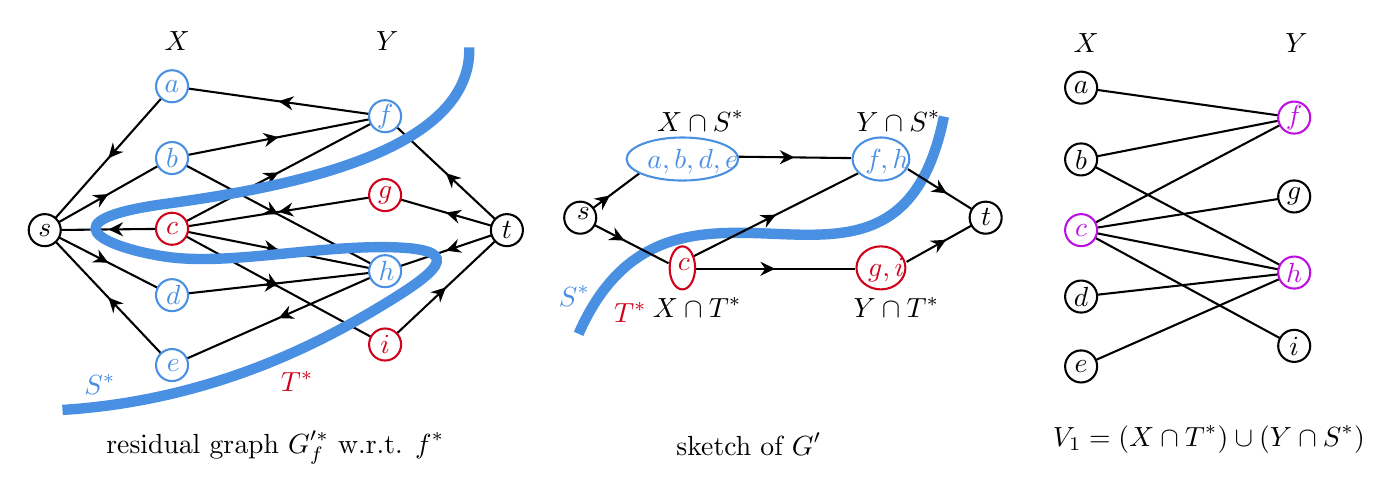
\begin{tikzpicture}[x=0.5pt,y=0.5pt,yscale=-1,xscale=1]
%uncomment if require: \path (0,327); %set diagram left start at 0, and has height of 327

%Straight Lines [id:da9104884328106918] 
\draw    (110.68,50.09) -- (18.68,154.07) ;
\draw [shift={(64.68,102.08)}, rotate = 311.5] [fill={rgb, 255:red, 0; green, 0; blue, 0 }  ][line width=0.08]  [draw opacity=0] (10.72,-5.15) -- (0,0) -- (10.72,5.15) -- (7.12,0) -- cycle    ;
%Straight Lines [id:da7681874141811359] 
\draw    (110.68,101.97) -- (18.68,154.07) ;
\draw [shift={(64.68,128.02)}, rotate = 150.48] [fill={rgb, 255:red, 0; green, 0; blue, 0 }  ][line width=0.08]  [draw opacity=0] (10.72,-5.15) -- (0,0) -- (10.72,5.15) -- (7.12,0) -- cycle    ;
%Straight Lines [id:da7226320448766448] 
\draw    (110.68,153.07) -- (18.68,154.07) ;
\draw [shift={(64.68,153.57)}, rotate = 359.38] [fill={rgb, 255:red, 0; green, 0; blue, 0 }  ][line width=0.08]  [draw opacity=0] (10.72,-5.15) -- (0,0) -- (10.72,5.15) -- (7.12,0) -- cycle    ;
%Straight Lines [id:da49080721425324236] 
\draw    (110.68,201.07) -- (18.68,154.07) ;
\draw [shift={(64.68,177.57)}, rotate = 207.06] [fill={rgb, 255:red, 0; green, 0; blue, 0 }  ][line width=0.08]  [draw opacity=0] (10.72,-5.15) -- (0,0) -- (10.72,5.15) -- (7.12,0) -- cycle    ;
%Straight Lines [id:da47091521890310684] 
\draw    (110.68,251.58) -- (18.68,154.07) ;
\draw [shift={(64.68,202.82)}, rotate = 406.65999999999997] [fill={rgb, 255:red, 0; green, 0; blue, 0 }  ][line width=0.08]  [draw opacity=0] (10.72,-5.15) -- (0,0) -- (10.72,5.15) -- (7.12,0) -- cycle    ;
%Straight Lines [id:da15266436710879794] 
\draw    (352.68,154.07) -- (264.67,71.73) ;
\draw [shift={(308.67,112.9)}, rotate = 403.09000000000003] [fill={rgb, 255:red, 0; green, 0; blue, 0 }  ][line width=0.08]  [draw opacity=0] (10.72,-5.15) -- (0,0) -- (10.72,5.15) -- (7.12,0) -- cycle    ;
%Straight Lines [id:da0877880561036608] 
\draw    (352.68,154.07) -- (264.67,128.73) ;
\draw [shift={(308.67,141.4)}, rotate = 376.06] [fill={rgb, 255:red, 0; green, 0; blue, 0 }  ][line width=0.08]  [draw opacity=0] (10.72,-5.15) -- (0,0) -- (10.72,5.15) -- (7.12,0) -- cycle    ;
%Straight Lines [id:da1013780616185066] 
\draw    (352.68,154.07) -- (264.67,183.73) ;
\draw [shift={(308.67,168.9)}, rotate = 341.38] [fill={rgb, 255:red, 0; green, 0; blue, 0 }  ][line width=0.08]  [draw opacity=0] (10.72,-5.15) -- (0,0) -- (10.72,5.15) -- (7.12,0) -- cycle    ;
%Straight Lines [id:da6251395403106741] 
\draw    (352.68,154.07) -- (264.67,236.73) ;
\draw [shift={(308.67,195.4)}, rotate = 136.8] [fill={rgb, 255:red, 0; green, 0; blue, 0 }  ][line width=0.08]  [draw opacity=0] (10.72,-5.15) -- (0,0) -- (10.72,5.15) -- (7.12,0) -- cycle    ;
%Straight Lines [id:da6233481480623783] 
\draw    (921.67,72.73) -- (767.68,102.97) ;
%Straight Lines [id:da3790939323014558] 
\draw    (767.68,51.09) -- (921.67,72.73) ;
%Straight Lines [id:da555393377892622] 
\draw    (921.67,72.73) -- (767.68,154.07) ;
%Straight Lines [id:da17109149534540602] 
\draw    (921.67,184.73) -- (767.68,154.07) ;
%Straight Lines [id:da8491552224613422] 
\draw    (921.67,237.73) -- (767.68,154.07) ;
%Straight Lines [id:da6111412207445381] 
\draw    (921.67,129.73) -- (767.68,154.07) ;
%Straight Lines [id:da40246334963984653] 
\draw    (921.67,184.73) -- (767.68,202.07) ;
%Straight Lines [id:da8951096474536266] 
\draw    (921.67,184.73) -- (767.68,252.58) ;
%Straight Lines [id:da442507224234595] 
\draw    (921.67,184.73) -- (767.68,102.97) ;
%Shape: Ellipse [id:dp9133580928774087] 
\draw  [fill={rgb, 255:red, 255; green, 255; blue, 255 }  ,fill opacity=1 ] (756.1,252.58) .. controls (756.1,246.18) and (761.29,241) .. (767.68,241) .. controls (774.08,241) and (779.26,246.18) .. (779.26,252.58) .. controls (779.26,258.97) and (774.08,264.16) .. (767.68,264.16) .. controls (761.29,264.16) and (756.1,258.97) .. (756.1,252.58) -- cycle ;
%Shape: Ellipse [id:dp4005957609675306] 
\draw  [fill={rgb, 255:red, 255; green, 255; blue, 255 }  ,fill opacity=1 ] (756.1,102.97) .. controls (756.1,96.57) and (761.29,91.39) .. (767.68,91.39) .. controls (774.08,91.39) and (779.26,96.57) .. (779.26,102.97) .. controls (779.26,109.36) and (774.08,114.55) .. (767.68,114.55) .. controls (761.29,114.55) and (756.1,109.36) .. (756.1,102.97) -- cycle ;
%Shape: Ellipse [id:dp49214617921702164] 
\draw  [color={rgb, 255:red, 189; green, 16; blue, 224 }  ,draw opacity=1 ][fill={rgb, 255:red, 255; green, 255; blue, 255 }  ,fill opacity=1 ] (756.1,154.07) .. controls (756.1,147.67) and (761.29,142.49) .. (767.68,142.49) .. controls (774.08,142.49) and (779.26,147.67) .. (779.26,154.07) .. controls (779.26,160.46) and (774.08,165.65) .. (767.68,165.65) .. controls (761.29,165.65) and (756.1,160.46) .. (756.1,154.07) -- cycle ;
%Shape: Ellipse [id:dp8440754424343925] 
\draw  [fill={rgb, 255:red, 255; green, 255; blue, 255 }  ,fill opacity=1 ] (756.1,202.07) .. controls (756.1,195.68) and (761.29,190.49) .. (767.68,190.49) .. controls (774.08,190.49) and (779.26,195.68) .. (779.26,202.07) .. controls (779.26,208.47) and (774.08,213.65) .. (767.68,213.65) .. controls (761.29,213.65) and (756.1,208.47) .. (756.1,202.07) -- cycle ;
%Shape: Ellipse [id:dp20660183368429152] 
\draw  [fill={rgb, 255:red, 255; green, 255; blue, 255 }  ,fill opacity=1 ] (756.1,51.09) .. controls (756.1,44.7) and (761.29,39.51) .. (767.68,39.51) .. controls (774.08,39.51) and (779.26,44.7) .. (779.26,51.09) .. controls (779.26,57.49) and (774.08,62.67) .. (767.68,62.67) .. controls (761.29,62.67) and (756.1,57.49) .. (756.1,51.09) -- cycle ;
%Shape: Ellipse [id:dp4098192910838151] 
\draw  [color={rgb, 255:red, 189; green, 16; blue, 224 }  ,draw opacity=1 ][fill={rgb, 255:red, 255; green, 255; blue, 255 }  ,fill opacity=1 ] (910.09,72.73) .. controls (910.09,66.33) and (915.27,61.15) .. (921.67,61.15) .. controls (928.06,61.15) and (933.25,66.33) .. (933.25,72.73) .. controls (933.25,79.13) and (928.06,84.31) .. (921.67,84.31) .. controls (915.27,84.31) and (910.09,79.13) .. (910.09,72.73) -- cycle ;
%Shape: Ellipse [id:dp04818959761719954] 
\draw  [fill={rgb, 255:red, 255; green, 255; blue, 255 }  ,fill opacity=1 ] (910.09,129.73) .. controls (910.09,123.33) and (915.27,118.15) .. (921.67,118.15) .. controls (928.06,118.15) and (933.25,123.33) .. (933.25,129.73) .. controls (933.25,136.13) and (928.06,141.31) .. (921.67,141.31) .. controls (915.27,141.31) and (910.09,136.13) .. (910.09,129.73) -- cycle ;
%Shape: Ellipse [id:dp776083183452069] 
\draw  [color={rgb, 255:red, 189; green, 16; blue, 224 }  ,draw opacity=1 ][fill={rgb, 255:red, 255; green, 255; blue, 255 }  ,fill opacity=1 ] (910.09,184.73) .. controls (910.09,178.33) and (915.27,173.15) .. (921.67,173.15) .. controls (928.06,173.15) and (933.25,178.33) .. (933.25,184.73) .. controls (933.25,191.13) and (928.06,196.31) .. (921.67,196.31) .. controls (915.27,196.31) and (910.09,191.13) .. (910.09,184.73) -- cycle ;
%Shape: Ellipse [id:dp943943166831801] 
\draw  [fill={rgb, 255:red, 255; green, 255; blue, 255 }  ,fill opacity=1 ] (910.09,237.73) .. controls (910.09,231.33) and (915.27,226.15) .. (921.67,226.15) .. controls (928.06,226.15) and (933.25,231.33) .. (933.25,237.73) .. controls (933.25,244.13) and (928.06,249.31) .. (921.67,249.31) .. controls (915.27,249.31) and (910.09,244.13) .. (910.09,237.73) -- cycle ;
%Straight Lines [id:da2316107627226749] 
\draw    (264.67,71.73) -- (110.68,101.97) ;
\draw [shift={(187.67,86.85)}, rotate = 168.89] [fill={rgb, 255:red, 0; green, 0; blue, 0 }  ][line width=0.08]  [draw opacity=0] (10.72,-5.15) -- (0,0) -- (10.72,5.15) -- (7.12,0) -- cycle    ;
%Straight Lines [id:da18627772384857166] 
\draw    (110.68,50.09) -- (264.67,71.73) ;
\draw [shift={(187.67,60.91)}, rotate = 8] [fill={rgb, 255:red, 0; green, 0; blue, 0 }  ][line width=0.08]  [draw opacity=0] (10.72,-5.15) -- (0,0) -- (10.72,5.15) -- (7.12,0) -- cycle    ;
%Straight Lines [id:da0577243134049511] 
\draw    (264.67,71.73) -- (110.68,153.07) ;
\draw [shift={(187.67,112.4)}, rotate = 152.16] [fill={rgb, 255:red, 0; green, 0; blue, 0 }  ][line width=0.08]  [draw opacity=0] (10.72,-5.15) -- (0,0) -- (10.72,5.15) -- (7.12,0) -- cycle    ;
%Straight Lines [id:da5892851585558246] 
\draw    (264.67,183.73) -- (110.68,153.07) ;
\draw [shift={(187.67,168.4)}, rotate = 191.26] [fill={rgb, 255:red, 0; green, 0; blue, 0 }  ][line width=0.08]  [draw opacity=0] (10.72,-5.15) -- (0,0) -- (10.72,5.15) -- (7.12,0) -- cycle    ;
%Straight Lines [id:da3983360233296235] 
\draw    (264.67,236.73) -- (110.68,153.07) ;
\draw [shift={(187.67,194.9)}, rotate = 208.52] [fill={rgb, 255:red, 0; green, 0; blue, 0 }  ][line width=0.08]  [draw opacity=0] (10.72,-5.15) -- (0,0) -- (10.72,5.15) -- (7.12,0) -- cycle    ;
%Straight Lines [id:da6135696831152091] 
\draw    (264.67,128.73) -- (110.68,153.07) ;
\draw [shift={(187.67,140.9)}, rotate = 351.02] [fill={rgb, 255:red, 0; green, 0; blue, 0 }  ][line width=0.08]  [draw opacity=0] (10.72,-5.15) -- (0,0) -- (10.72,5.15) -- (7.12,0) -- cycle    ;
%Straight Lines [id:da9672640821433086] 
\draw    (264.67,183.73) -- (110.68,201.07) ;
\draw [shift={(187.67,192.4)}, rotate = 173.57] [fill={rgb, 255:red, 0; green, 0; blue, 0 }  ][line width=0.08]  [draw opacity=0] (10.72,-5.15) -- (0,0) -- (10.72,5.15) -- (7.12,0) -- cycle    ;
%Straight Lines [id:da7832805423777587] 
\draw    (264.67,183.73) -- (110.68,251.58) ;
\draw [shift={(187.67,217.65)}, rotate = 336.22] [fill={rgb, 255:red, 0; green, 0; blue, 0 }  ][line width=0.08]  [draw opacity=0] (10.72,-5.15) -- (0,0) -- (10.72,5.15) -- (7.12,0) -- cycle    ;
%Straight Lines [id:da1526453815123745] 
\draw    (264.67,183.73) -- (110.68,101.97) ;
\draw [shift={(187.67,142.85)}, rotate = 207.97] [fill={rgb, 255:red, 0; green, 0; blue, 0 }  ][line width=0.08]  [draw opacity=0] (10.72,-5.15) -- (0,0) -- (10.72,5.15) -- (7.12,0) -- cycle    ;
%Shape: Ellipse [id:dp6654229458693389] 
\draw  [color={rgb, 255:red, 74; green, 144; blue, 226 }  ,draw opacity=1 ][fill={rgb, 255:red, 255; green, 255; blue, 255 }  ,fill opacity=1 ] (99.1,251.58) .. controls (99.1,245.18) and (104.29,240) .. (110.68,240) .. controls (117.08,240) and (122.26,245.18) .. (122.26,251.58) .. controls (122.26,257.97) and (117.08,263.16) .. (110.68,263.16) .. controls (104.29,263.16) and (99.1,257.97) .. (99.1,251.58) -- cycle ;
%Shape: Ellipse [id:dp12431995068279444] 
\draw  [color={rgb, 255:red, 74; green, 144; blue, 226 }  ,draw opacity=1 ][fill={rgb, 255:red, 255; green, 255; blue, 255 }  ,fill opacity=1 ] (99.1,101.97) .. controls (99.1,95.57) and (104.29,90.39) .. (110.68,90.39) .. controls (117.08,90.39) and (122.26,95.57) .. (122.26,101.97) .. controls (122.26,108.36) and (117.08,113.55) .. (110.68,113.55) .. controls (104.29,113.55) and (99.1,108.36) .. (99.1,101.97) -- cycle ;
%Shape: Ellipse [id:dp20588104884103686] 
\draw  [color={rgb, 255:red, 208; green, 2; blue, 27 }  ,draw opacity=1 ][fill={rgb, 255:red, 255; green, 255; blue, 255 }  ,fill opacity=1 ] (99.1,153.07) .. controls (99.1,146.67) and (104.29,141.49) .. (110.68,141.49) .. controls (117.08,141.49) and (122.26,146.67) .. (122.26,153.07) .. controls (122.26,159.46) and (117.08,164.65) .. (110.68,164.65) .. controls (104.29,164.65) and (99.1,159.46) .. (99.1,153.07) -- cycle ;
%Shape: Ellipse [id:dp7769132906685045] 
\draw  [color={rgb, 255:red, 74; green, 144; blue, 226 }  ,draw opacity=1 ][fill={rgb, 255:red, 255; green, 255; blue, 255 }  ,fill opacity=1 ] (99.1,201.07) .. controls (99.1,194.68) and (104.29,189.49) .. (110.68,189.49) .. controls (117.08,189.49) and (122.26,194.68) .. (122.26,201.07) .. controls (122.26,207.47) and (117.08,212.65) .. (110.68,212.65) .. controls (104.29,212.65) and (99.1,207.47) .. (99.1,201.07) -- cycle ;
%Shape: Ellipse [id:dp9884072609577427] 
\draw  [color={rgb, 255:red, 74; green, 144; blue, 226 }  ,draw opacity=1 ][fill={rgb, 255:red, 255; green, 255; blue, 255 }  ,fill opacity=1 ] (99.1,50.09) .. controls (99.1,43.7) and (104.29,38.51) .. (110.68,38.51) .. controls (117.08,38.51) and (122.26,43.7) .. (122.26,50.09) .. controls (122.26,56.49) and (117.08,61.67) .. (110.68,61.67) .. controls (104.29,61.67) and (99.1,56.49) .. (99.1,50.09) -- cycle ;
%Shape: Ellipse [id:dp42354463997423675] 
\draw  [color={rgb, 255:red, 74; green, 144; blue, 226 }  ,draw opacity=1 ][fill={rgb, 255:red, 255; green, 255; blue, 255 }  ,fill opacity=1 ] (253.09,71.73) .. controls (253.09,65.33) and (258.27,60.15) .. (264.67,60.15) .. controls (271.06,60.15) and (276.25,65.33) .. (276.25,71.73) .. controls (276.25,78.13) and (271.06,83.31) .. (264.67,83.31) .. controls (258.27,83.31) and (253.09,78.13) .. (253.09,71.73) -- cycle ;
%Shape: Ellipse [id:dp6229410956087476] 
\draw  [color={rgb, 255:red, 208; green, 2; blue, 27 }  ,draw opacity=1 ][fill={rgb, 255:red, 255; green, 255; blue, 255 }  ,fill opacity=1 ] (253.09,128.73) .. controls (253.09,122.33) and (258.27,117.15) .. (264.67,117.15) .. controls (271.06,117.15) and (276.25,122.33) .. (276.25,128.73) .. controls (276.25,135.13) and (271.06,140.31) .. (264.67,140.31) .. controls (258.27,140.31) and (253.09,135.13) .. (253.09,128.73) -- cycle ;
%Shape: Ellipse [id:dp791442075919042] 
\draw  [color={rgb, 255:red, 74; green, 144; blue, 226 }  ,draw opacity=1 ][fill={rgb, 255:red, 255; green, 255; blue, 255 }  ,fill opacity=1 ] (253.09,183.73) .. controls (253.09,177.33) and (258.27,172.15) .. (264.67,172.15) .. controls (271.06,172.15) and (276.25,177.33) .. (276.25,183.73) .. controls (276.25,190.13) and (271.06,195.31) .. (264.67,195.31) .. controls (258.27,195.31) and (253.09,190.13) .. (253.09,183.73) -- cycle ;
%Shape: Ellipse [id:dp004238859938154427] 
\draw  [color={rgb, 255:red, 208; green, 2; blue, 27 }  ,draw opacity=1 ][fill={rgb, 255:red, 255; green, 255; blue, 255 }  ,fill opacity=1 ] (253.09,236.73) .. controls (253.09,230.33) and (258.27,225.15) .. (264.67,225.15) .. controls (271.06,225.15) and (276.25,230.33) .. (276.25,236.73) .. controls (276.25,243.13) and (271.06,248.31) .. (264.67,248.31) .. controls (258.27,248.31) and (253.09,243.13) .. (253.09,236.73) -- cycle ;
%Shape: Ellipse [id:dp22397680523687857] 
\draw  [fill={rgb, 255:red, 255; green, 255; blue, 255 }  ,fill opacity=1 ] (7.1,154.07) .. controls (7.1,147.67) and (12.29,142.49) .. (18.68,142.49) .. controls (25.08,142.49) and (30.26,147.67) .. (30.26,154.07) .. controls (30.26,160.46) and (25.08,165.65) .. (18.68,165.65) .. controls (12.29,165.65) and (7.1,160.46) .. (7.1,154.07) -- cycle ;
%Shape: Ellipse [id:dp24170948792038305] 
\draw  [fill={rgb, 255:red, 255; green, 255; blue, 255 }  ,fill opacity=1 ] (341.1,154.07) .. controls (341.1,147.67) and (346.29,142.49) .. (352.68,142.49) .. controls (359.08,142.49) and (364.26,147.67) .. (364.26,154.07) .. controls (364.26,160.46) and (359.08,165.65) .. (352.68,165.65) .. controls (346.29,165.65) and (341.1,160.46) .. (341.1,154.07) -- cycle ;
%Curve Lines [id:da6554198471738361] 
\draw [color={rgb, 255:red, 74; green, 144; blue, 226 }  ,draw opacity=1 ][line width=3.75]    (325.5,22) .. controls (327.5,98) and (193.32,123.23) .. (106.5,135) .. controls (19.68,146.77) and (60.5,166) .. (104.5,173) .. controls (148.5,180) and (210.35,165.74) .. (265.42,166.37) .. controls (320.5,167) and (307.5,181) .. (266.51,206.07) .. controls (225.52,231.14) and (144.5,277) .. (31.5,284) ;
%Curve Lines [id:da1215081826403992] 
\draw [color={rgb, 255:red, 74; green, 144; blue, 226 }  ,draw opacity=1 ][line width=3.75]    (404.5,229) .. controls (473.5,72) and (633.5,246) .. (668.5,72) ;
%Straight Lines [id:da21919794802744808] 
\draw    (405.68,145.07) -- (448.5,113) ;
\draw [shift={(427.09,129.03)}, rotate = 503.17] [fill={rgb, 255:red, 0; green, 0; blue, 0 }  ][line width=0.08]  [draw opacity=0] (10.72,-5.15) -- (0,0) -- (10.72,5.15) -- (7.12,0) -- cycle    ;
%Straight Lines [id:da6571553793489531] 
\draw    (405.68,145.07) -- (469.5,178) ;
\draw [shift={(437.59,161.53)}, rotate = 207.29] [fill={rgb, 255:red, 0; green, 0; blue, 0 }  ][line width=0.08]  [draw opacity=0] (10.72,-5.15) -- (0,0) -- (10.72,5.15) -- (7.12,0) -- cycle    ;
%Straight Lines [id:da4584473388976602] 
\draw    (519.5,101) -- (601.5,102) ;
\draw [shift={(560.5,101.5)}, rotate = 180.7] [fill={rgb, 255:red, 0; green, 0; blue, 0 }  ][line width=0.08]  [draw opacity=0] (10.72,-5.15) -- (0,0) -- (10.72,5.15) -- (7.12,0) -- cycle    ;
%Straight Lines [id:da6647190591773025] 
\draw    (488.5,182) -- (604.5,182) ;
\draw [shift={(546.5,182)}, rotate = 180] [fill={rgb, 255:red, 0; green, 0; blue, 0 }  ][line width=0.08]  [draw opacity=0] (10.72,-5.15) -- (0,0) -- (10.72,5.15) -- (7.12,0) -- cycle    ;
%Straight Lines [id:da26541070418887813] 
\draw    (487.5,173) -- (606.5,113) ;
\draw [shift={(547,143)}, rotate = 513.24] [fill={rgb, 255:red, 0; green, 0; blue, 0 }  ][line width=0.08]  [draw opacity=0] (10.72,-5.15) -- (0,0) -- (10.72,5.15) -- (7.12,0) -- cycle    ;
%Straight Lines [id:da11614592706967275] 
\draw    (642.5,110) -- (698.68,145.07) ;
\draw [shift={(670.59,127.53)}, rotate = 211.97] [fill={rgb, 255:red, 0; green, 0; blue, 0 }  ][line width=0.08]  [draw opacity=0] (10.72,-5.15) -- (0,0) -- (10.72,5.15) -- (7.12,0) -- cycle    ;
%Straight Lines [id:da8549744166457882] 
\draw    (641.5,177) -- (698.68,145.07) ;
\draw [shift={(670.09,161.03)}, rotate = 510.82] [fill={rgb, 255:red, 0; green, 0; blue, 0 }  ][line width=0.08]  [draw opacity=0] (10.72,-5.15) -- (0,0) -- (10.72,5.15) -- (7.12,0) -- cycle    ;
%Shape: Ellipse [id:dp8482659470468372] 
\draw  [fill={rgb, 255:red, 255; green, 255; blue, 255 }  ,fill opacity=1 ] (394.1,145.07) .. controls (394.1,138.67) and (399.29,133.49) .. (405.68,133.49) .. controls (412.08,133.49) and (417.26,138.67) .. (417.26,145.07) .. controls (417.26,151.46) and (412.08,156.65) .. (405.68,156.65) .. controls (399.29,156.65) and (394.1,151.46) .. (394.1,145.07) -- cycle ;
%Shape: Ellipse [id:dp5378543578011696] 
\draw  [fill={rgb, 255:red, 255; green, 255; blue, 255 }  ,fill opacity=1 ] (687.1,145.07) .. controls (687.1,138.67) and (692.29,133.49) .. (698.68,133.49) .. controls (705.08,133.49) and (710.26,138.67) .. (710.26,145.07) .. controls (710.26,151.46) and (705.08,156.65) .. (698.68,156.65) .. controls (692.29,156.65) and (687.1,151.46) .. (687.1,145.07) -- cycle ;

% Text Node
\draw (767.68,252.58) node   [align=left] {$\displaystyle e$};
% Text Node
\draw (767.68,102.97) node   [align=left] {$\displaystyle b$};
% Text Node
\draw (767.68,154.07) node  [color={rgb, 255:red, 189; green, 16; blue, 224 }  ,opacity=1 ] [align=left] {$\displaystyle c$};
% Text Node
\draw (767.68,202.07) node   [align=left] {$\displaystyle d$};
% Text Node
\draw (767.68,51.09) node   [align=left] {$\displaystyle a$};
% Text Node
\draw (921.67,72.73) node  [color={rgb, 255:red, 189; green, 16; blue, 224 }  ,opacity=1 ] [align=left] {$\displaystyle f$};
% Text Node
\draw (921.67,129.73) node   [align=left] {$\displaystyle g$};
% Text Node
\draw (921.67,184.73) node  [color={rgb, 255:red, 189; green, 16; blue, 224 }  ,opacity=1 ] [align=left] {$\displaystyle h$};
% Text Node
\draw (921.67,237.73) node   [align=left] {$\displaystyle i$};
% Text Node
\draw (760,9.5) node [anchor=north west][inner sep=0.75pt]   [align=left] {$\displaystyle X$};
% Text Node
\draw (913,9.5) node [anchor=north west][inner sep=0.75pt]   [align=left] {$\displaystyle Y$};
% Text Node
\draw (111.68,251.58) node  [color={rgb, 255:red, 74; green, 144; blue, 226 }  ,opacity=1 ] [align=left] {$\displaystyle e$};
% Text Node
\draw (110.68,101.97) node  [color={rgb, 255:red, 74; green, 144; blue, 226 }  ,opacity=1 ] [align=left] {$\displaystyle b$};
% Text Node
\draw (110.68,153.07) node  [color={rgb, 255:red, 208; green, 2; blue, 27 }  ,opacity=1 ] [align=left] {$\displaystyle c$};
% Text Node
\draw (111.68,201.07) node  [color={rgb, 255:red, 74; green, 144; blue, 226 }  ,opacity=1 ] [align=left] {$\displaystyle d$};
% Text Node
\draw (110.68,50.09) node  [color={rgb, 255:red, 74; green, 144; blue, 226 }  ,opacity=1 ] [align=left] {$\displaystyle a$};
% Text Node
\draw (264.67,71.73) node  [color={rgb, 255:red, 74; green, 144; blue, 226 }  ,opacity=1 ] [align=left] {$\displaystyle f$};
% Text Node
\draw (459,65.67) node [anchor=north west][inner sep=0.75pt]   [align=left] {$\displaystyle X\cap S^{*}$};
% Text Node
\draw (264.67,128.73) node  [color={rgb, 255:red, 208; green, 2; blue, 27 }  ,opacity=1 ] [align=left] {$\displaystyle g$};
% Text Node
\draw (265.67,183.73) node  [color={rgb, 255:red, 74; green, 144; blue, 226 }  ,opacity=1 ] [align=left] {$\displaystyle h$};
% Text Node
\draw (264.67,236.73) node  [color={rgb, 255:red, 208; green, 2; blue, 27 }  ,opacity=1 ] [align=left] {$\displaystyle i$};
% Text Node
\draw (103,8.5) node [anchor=north west][inner sep=0.75pt]   [align=left] {$\displaystyle X$};
% Text Node
\draw (256,8.5) node [anchor=north west][inner sep=0.75pt]   [align=left] {$\displaystyle Y$};
% Text Node
\draw (18.68,154.07) node  [color={rgb, 255:red, 0; green, 0; blue, 0 }  ,opacity=1 ] [align=left] {$\displaystyle s$};
% Text Node
\draw (352.68,154.07) node  [color={rgb, 255:red, 0; green, 0; blue, 0 }  ,opacity=1 ] [align=left] {$\displaystyle t$};
% Text Node
\draw (61,297) node [anchor=north west][inner sep=0.75pt]   [align=left] {residual graph $\displaystyle G^{\prime *}_{f}$ w.r.t. $\displaystyle f^{*}$};
% Text Node
\draw (45,256) node [anchor=north west][inner sep=0.75pt]   [align=left] {$\displaystyle \textcolor[rgb]{0.29,0.56,0.89}{S}\textcolor[rgb]{0.29,0.56,0.89}{^{*}}$};
% Text Node
\draw (187,254) node [anchor=north west][inner sep=0.75pt]   [align=left] {$\displaystyle \textcolor[rgb]{0.82,0.01,0.11}{T}\textcolor[rgb]{0.82,0.01,0.11}{^{*}}$};
% Text Node
\draw (456,200.33) node [anchor=north west][inner sep=0.75pt]   [align=left] {$\displaystyle X\cap T^{*}$};
% Text Node
\draw (603,65.67) node [anchor=north west][inner sep=0.75pt]   [align=left] {$\displaystyle Y\cap S^{*}$};
% Text Node
\draw (601,200.34) node [anchor=north west][inner sep=0.75pt]   [align=left] {$\displaystyle Y\cap T^{*}$};
% Text Node
\draw (745,293) node [anchor=north west][inner sep=0.75pt]   [align=left] { $\displaystyle V_{1} =\left( X\cap T^{*}\right) \cup \left( Y\cap S^{*}\right)$};
% Text Node
\draw  [color={rgb, 255:red, 74; green, 144; blue, 226 }  ,draw opacity=1 ]  (479.5, 102.67) circle [x radius= 40.31, y radius= 15.56]   ;
\draw (452,93.67) node [anchor=north west][inner sep=0.75pt]   [align=left] {$\displaystyle \textcolor[rgb]{0.29,0.56,0.89}{a,b,d,e}$};
% Text Node
\draw  [color={rgb, 255:red, 208; green, 2; blue, 27 }  ,draw opacity=1 ]  (479.5, 181.34) circle [x radius= 9.19, y radius= 15.56]   ;
\draw (474,172.34) node [anchor=north west][inner sep=0.75pt]   [align=left] {$\displaystyle \textcolor[rgb]{0.82,0.01,0.11}{c}$};
% Text Node
\draw  [color={rgb, 255:red, 74; green, 144; blue, 226 }  ,draw opacity=1 ]  (623, 102.67) circle [x radius= 20.51, y radius= 15.56]   ;
\draw (609.5,93.67) node [anchor=north west][inner sep=0.75pt]   [align=left] {$\displaystyle \textcolor[rgb]{0.29,0.56,0.89}{f,h}$};
% Text Node
\draw  [color={rgb, 255:red, 208; green, 2; blue, 27 }  ,draw opacity=1 ]  (623, 181.34) circle [x radius= 17.68, y radius= 15.56]   ;
\draw (611.5,172.34) node [anchor=north west][inner sep=0.75pt]   [align=left] {$\displaystyle \textcolor[rgb]{0.82,0.01,0.11}{g,i}$};
% Text Node
\draw (401,135.5) node [anchor=north west][inner sep=0.75pt]   [align=left] {$\displaystyle s$};
% Text Node
\draw (388,192) node [anchor=north west][inner sep=0.75pt]   [align=left] {$\displaystyle \textcolor[rgb]{0.29,0.56,0.89}{S}\textcolor[rgb]{0.29,0.56,0.89}{^{*}}$};
% Text Node
\draw (428,204) node [anchor=north west][inner sep=0.75pt]   [align=left] {$\displaystyle \textcolor[rgb]{0.82,0.01,0.11}{T}\textcolor[rgb]{0.82,0.01,0.11}{^{*}}$};
% Text Node
\draw (693.18,136.07) node [anchor=north west][inner sep=0.75pt]   [align=left] {$\displaystyle t$};
% Text Node
\draw (473,298.5) node [anchor=north west][inner sep=0.75pt]   [align=left] {sketch of $\displaystyle G'$};


\end{tikzpicture}

